\documentclass[xcolor=table]{beamer}

\usepackage[american]{babel} % ngerman / american
\usepackage[utf8]{inputenc} % For "Umlaut"s
\usepackage{makecell}
\usepackage[table]{xcolor}
\definecolor{Gray}{gray}{0.8}
\definecolor{DarkRed}{rgb}{.7,0,0}
\definecolor{Red}{rgb}{.9,0,0}
\definecolor{DarkGreen}{rgb}{0,.7,0}
\definecolor{Green}{rgb}{0,.9,0}
\usepackage{booktabs}
\setlength{\aboverulesep}{0pt}
\setlength{\belowrulesep}{0pt}
\setbeamertemplate{caption}[numbered]
\usepackage{tabularx,colortbl}
\usepackage{minted} % Code highlighting
\usemintedstyle{default} % Set style of code highlighting
\usepackage{rotating}
\usepackage{soul} % for strikethrough text: \st{Text}
\usepackage[export]{adjustbox} % for figures:
% \includegraphics[width=.6\textwidth,<left/right/center>]{example-image}
\usepackage{csquotes}
\usepackage[strict]{changepage}
\usepackage{framed}
\usepackage{booktabs}

%--Progress Bar Setup
\usepackage{tikz}
\usetikzlibrary{calc}
\definecolor{pbblue}{HTML}{0A75A8}% color for the progress bar and the circle
\makeatletter
\def\progressbar@progressbar{} % the progress bar
\newcount\progressbar@tmpcounta% auxiliary counter
\newcount\progressbar@tmpcountb% auxiliary counter
\newdimen\progressbar@pbht %progressbar height
\newdimen\progressbar@pbwd %progressbar width
\newdimen\progressbar@rcircle % radius for the circle
\newdimen\progressbar@tmpdim % auxiliary dimension

\progressbar@pbwd=1.1\linewidth
\progressbar@pbht=1pt
\progressbar@rcircle=2.5pt

% the progress bar
\def\progressbar@progressbar{% 

    \progressbar@tmpcounta=\insertframenumber
    \progressbar@tmpcountb=\inserttotalframenumber
    \progressbar@tmpdim=\progressbar@pbwd
    \multiply\progressbar@tmpdim by \progressbar@tmpcounta
    \divide\progressbar@tmpdim by \progressbar@tmpcountb

  \begin{tikzpicture}
    \draw[pbblue!30,line width=\progressbar@pbht]
      (0pt, 0pt) -- ++ (\progressbar@pbwd,0pt);

    \filldraw[pbblue!30] %
      (\the\dimexpr\progressbar@tmpdim-\progressbar@rcircle\relax, .5\progressbar@pbht) circle (\progressbar@rcircle);

    \node[draw=pbblue!30,text width=3.5em,align=center,inner sep=1pt,
      text=pbblue!70,anchor=east] at (0,0) {\insertframenumber/\inserttotalframenumber};
  \end{tikzpicture}%
}

\addtobeamertemplate{headline}{}
{%
  \begin{beamercolorbox}[wd=\paperwidth,ht=4ex,center,dp=1ex]{white}%
    \progressbar@progressbar%
  \end{beamercolorbox}%
}
\makeatother
%--

%--Fancy Quote Setup
\definecolor{formalshade}{rgb}{0.95,0.95,1}
\definecolor{darkblue}{rgb}{0.5,0.8,0.9}

\newenvironment{formal}{%
  \def\FrameCommand{%
    \hspace{1pt}%
    {\color{darkblue}\vrule width 2pt}%
    {\color{formalshade}\vrule width 4pt}%
    \colorbox{formalshade}%
  }%
  \MakeFramed{\advance\hsize-\width\FrameRestore}%
  \noindent\hspace{-4.55pt}% disable indenting first paragraph
  \begin{adjustwidth}{}{7pt}%
  \vspace{2pt}\vspace{2pt}%
}
{%
  \vspace{2pt}\end{adjustwidth}\endMakeFramed%
}
%--

% There are many different themes available for Beamer. A comprehensive list with examples is given here: http://deic.uab.es/~iblanes/beamer_gallery/index_by_theme.html
% You can uncomment the themes below if you would like to use a different one:
%\usetheme{AnnArbor}
%\usetheme{Antibes}
%\usetheme{Bergen}
%\usetheme{Berkeley}
%\usetheme{Berlin}
%\usetheme{Boadilla}
%\usetheme{boxes}
%\usetheme{CambridgeUS}
%\usetheme{Copenhagen}
%\usetheme{Darmstadt}
%\usetheme{default}
%\usetheme{Frankfurt}
\usetheme{Goettingen}
%\usetheme{Hannover}
%\usetheme{Ilmenau}
%\usetheme{JuanLesPins}
%\usetheme{Luebeck}
%\usetheme{Madrid}
%\usetheme{Malmoe}
%\usetheme{Marburg}
%\usetheme{Montpellier}
%\usetheme{PaloAlto}
%\usetheme{Pittsburgh}
%\usetheme{Rochester}
%\usetheme{Singapore}
%\usetheme{Szeged}
%\usetheme{Warsaw}

\title{Confusing Concurrency}

% A subtitle is optional and this may be deleted
\subtitle{RxJava in Action}

\author{Moritz Richter, Tim Wedde}
% - Give the names in the same order as the appear in the paper.
% - Use the \inst{?} command only if the authors have different
%   affiliation.

\institute {
  Enterprise System Whatever \\
  \bigskip
  FH Techniek en Logistiek \\
  Venlo
}
% - Use the \inst command only if there are several affiliations.
% - Keep it simple, no one is interested in your street address.

\date{\today}

% If you have a file called "university-logo-filename.xxx", where xxx
% is a graphic format that can be processed by latex or pdflatex,
% resp., then you can add a logo as follows:

% \pgfdeclareimage[height=0.5cm]{university-logo}{university-logo-filename}
% \logo{\pgfuseimage{university-logo}}

% Let's get started
% You can reveal the parts of a slide one at a time with the \pause command:
\begin{document}

\begin{frame}
  \titlepage
\end{frame}

% \begin{frame}{Contents}
%   \tableofcontents % You might wish to add the option [pausesections]
% \end{frame}

% Section and subsections will appear in the presentation overview and table of contents.

\section{Intro}\label{sec:intro}

\begin{frame}{What is RxJava?}
	\begin{figure}[h]
		
\includegraphics[width=0.5\textwidth,page=1]{gfx/rx_logo}
	\end{figure}
\end{frame}

\begin{frame}{Types of Concurrency}
	\begin{figure}[h]
		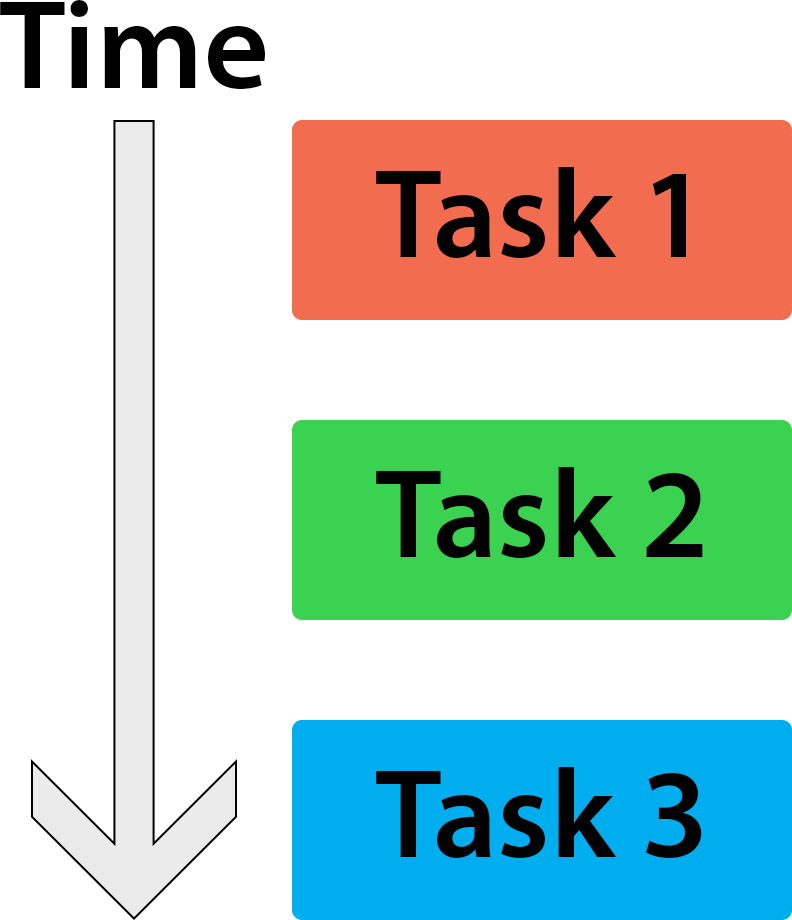
\includegraphics[width=0.6\textwidth,page=1]{gfx/single_threaded_nowait}
	\end{figure}
\end{frame}

\begin{frame}{Types of Concurrency}
	\begin{figure}[h]
		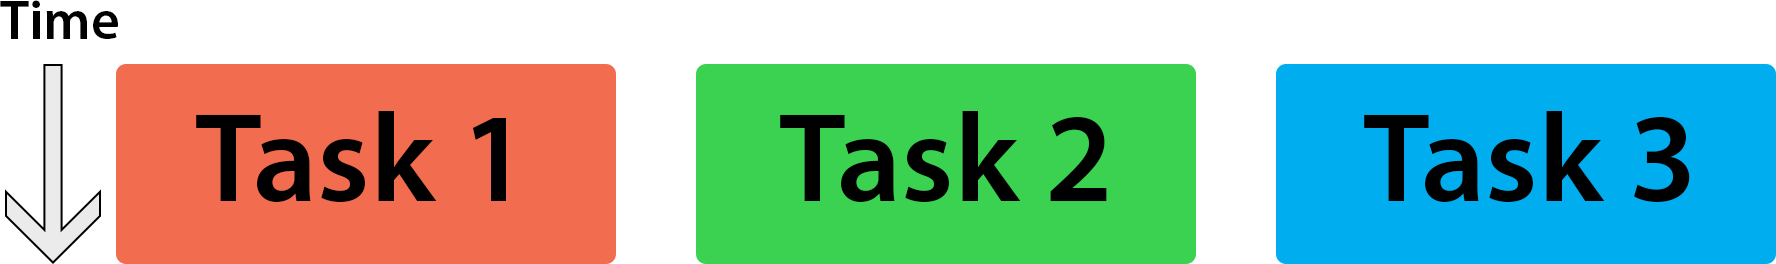
\includegraphics[width=1.0\textwidth,page=1]{gfx/multi_threaded}
	\end{figure}
\end{frame}

\begin{frame}{Types of Concurrency}
	\begin{figure}[h]
		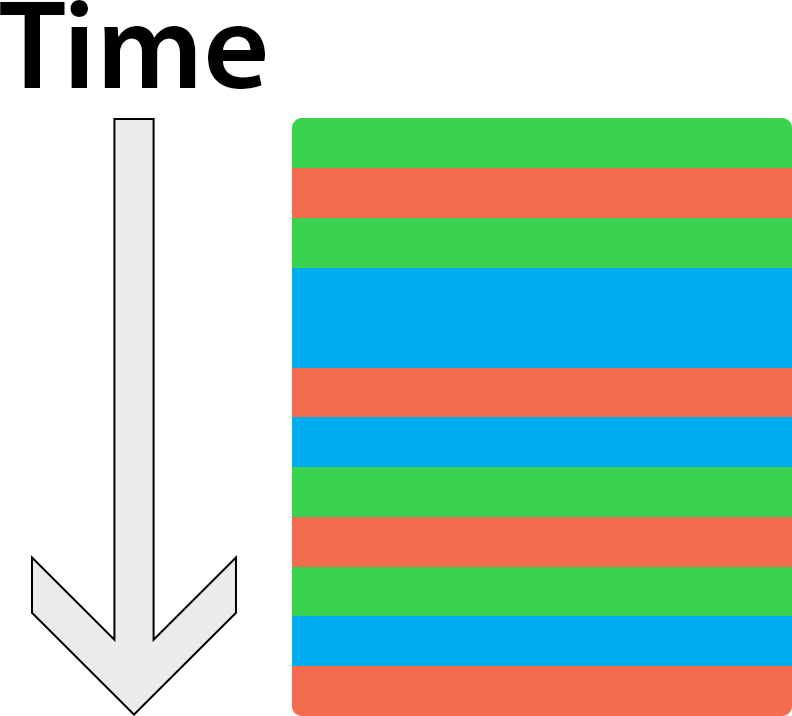
\includegraphics[width=0.7\textwidth,page=1]{gfx/asynchronous_nowait}
	\end{figure}
\end{frame}

\begin{frame}{Types of Concurrency}
	\begin{figure}[h]
		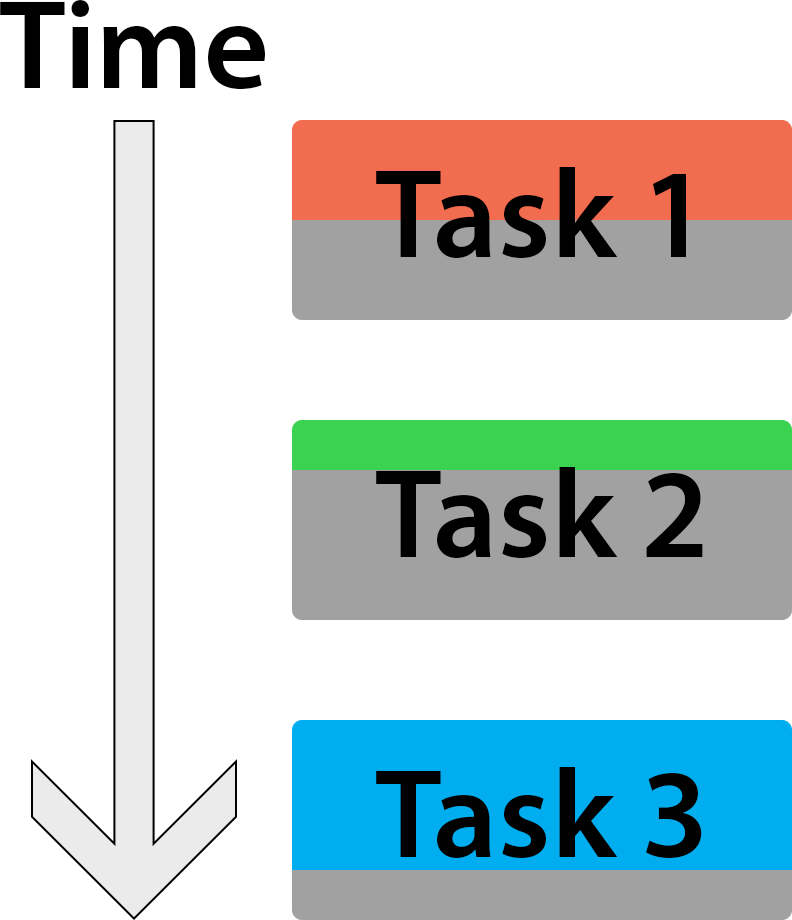
\includegraphics[width=0.6\textwidth,page=1]{gfx/single_threaded_wait}
	\end{figure}
\end{frame}

\begin{frame}[fragile]{Sequential Processing}
    \begin{minted}{python}
                try:
                    for item in collection:
    onNext() ->         doWithAndWaitFor(item)
                except Exception e:
   onError() ->     panic(e)

onComplete() -> cleanup()
    \end{minted}
\end{frame}

\begin{frame}{Types of Concurrency}
	\begin{figure}[h]
		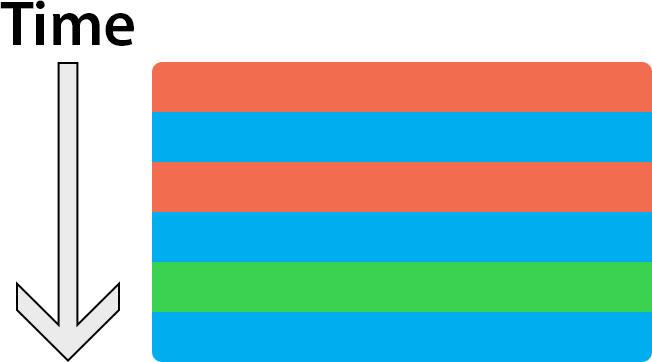
\includegraphics[width=0.7\textwidth,page=1]{gfx/asynchronous_wait}
	\end{figure}
\end{frame}

\begin{frame}{Callback Hell}
	\begin{figure}[h]
		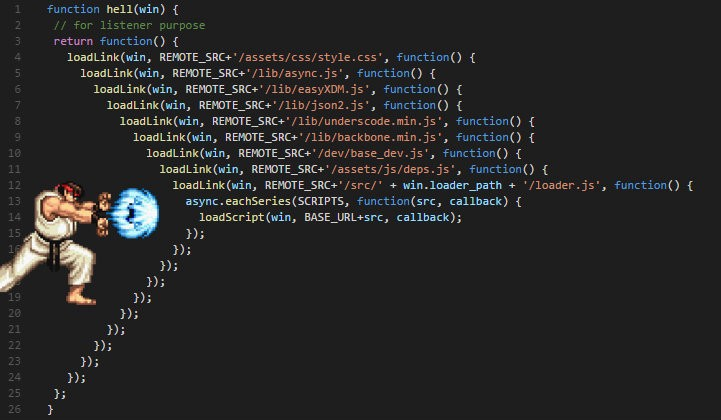
\includegraphics[width=1.0\textwidth,page=1]{gfx/callback_hadouken}
	\end{figure}
\end{frame}

\begin{frame}{Callback Hell - Dante's Inferno}
	\begin{figure}[h]
		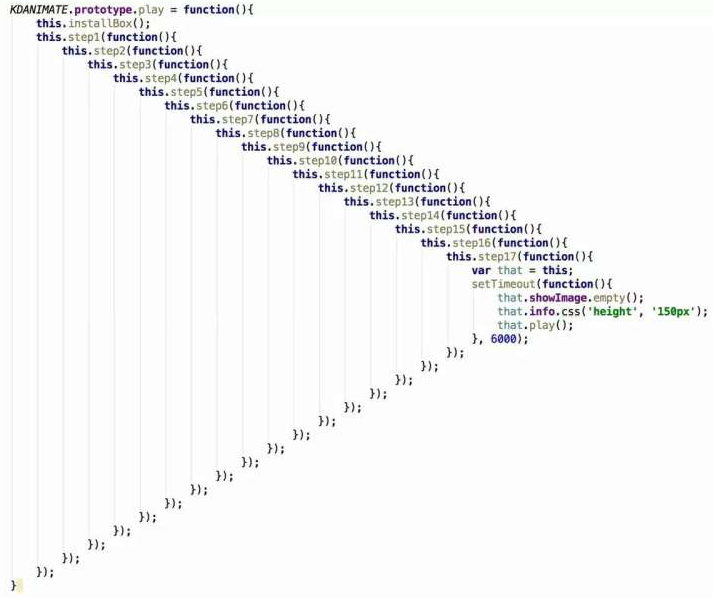
\includegraphics[width=0.9\textwidth,page=1]{gfx/extreme_callback}
	\end{figure}
\end{frame}


\section{RxJava}
\begin{frame}{Observer to the Rescue!}
	\begin{figure}[h]
		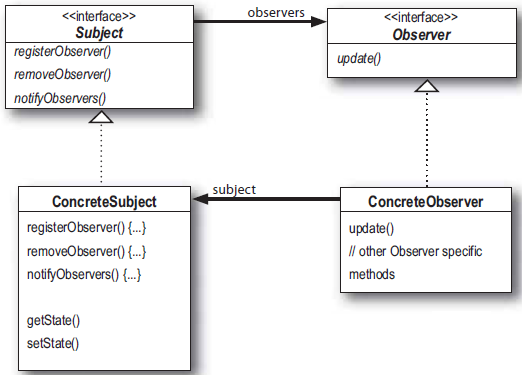
\includegraphics[width=1.0\textwidth,page=1]{gfx/observer_pattern}
	\end{figure}
\end{frame}

\begin{frame}{RxJava Observables}
    \centering
    \begin{tabular}{*3l}
        \toprule
        \textbf{Event} & \textbf{Iterable} & \textbf{Observable} \\
        \midrule
        retrieve data & \texttt{T next()} & \texttt{onNext(T)} \\
        discover error & \texttt{throws Ex.} & \cellcolor{green!50} \texttt{onError(Ex.)} \\
        complete & \texttt{!hasNext()} & \cellcolor{green!50} \texttt{onCompleted()} \\
        \bottomrule
    \end{tabular}
\end{frame}

\begin{frame}{What is RxJava?}
    \centering
    \Large
    \textbf{RxJava's objective is to work on discrete values that are emitted over time (streams), using a push-based architecture.}\\
    \bigskip
    $\rightarrow$ Reactive Programming $\leftarrow$
\end{frame}

\subsection{Streams in Java 8+}\label{sec:java}
\begin{frame}[fragile]{{\nameref{sec:java}}}
  \begin{minted}{java}
List<String> myList =
    Arrays.asList("a1", "a2", "b1", "c2", "c1");

myList
    .stream()
    .filter(s -> s.startsWith("c"))
    .map(String::toUpperCase)
    .sorted()
    .forEach(System.out::println);
  \end{minted}
\end{frame}

\begin{frame}{{\nameref{sec:java}}}
	\begin{itemize}
		\item Pull-based
        \item Single-Use, no forking or reusing
        \item No merging
        \item No time-based operations
	\end{itemize}
\end{frame}

\begin{frame}[fragile]{Back to the [Completable]Future?}
  \begin{minted}{java}
CompletableFuture<String> helloText =
    CompletableFuture.supplyAsync(() -> {
        TimeUnit.SECONDS.sleep(1);
        return "World";
    }).thenApply(name -> {
        return "Hello, " + name + "!";
    }).thenApply(text -> {
        return text + " This is callback chaining!";
    });

System.out.println(helloText.get());
  \end{minted}
\end{frame}

\subsection{Functional Progr.}
\begin{frame}{Functional Programming}
	\begin{itemize}
        \item No side effects
        \item No mutating state
        \item Arbitrary data
	\end{itemize}
\end{frame}

\section{Stream Operators}\label{sec:rxjava}
\begin{frame}{concat()}
	\begin{figure}[h]
		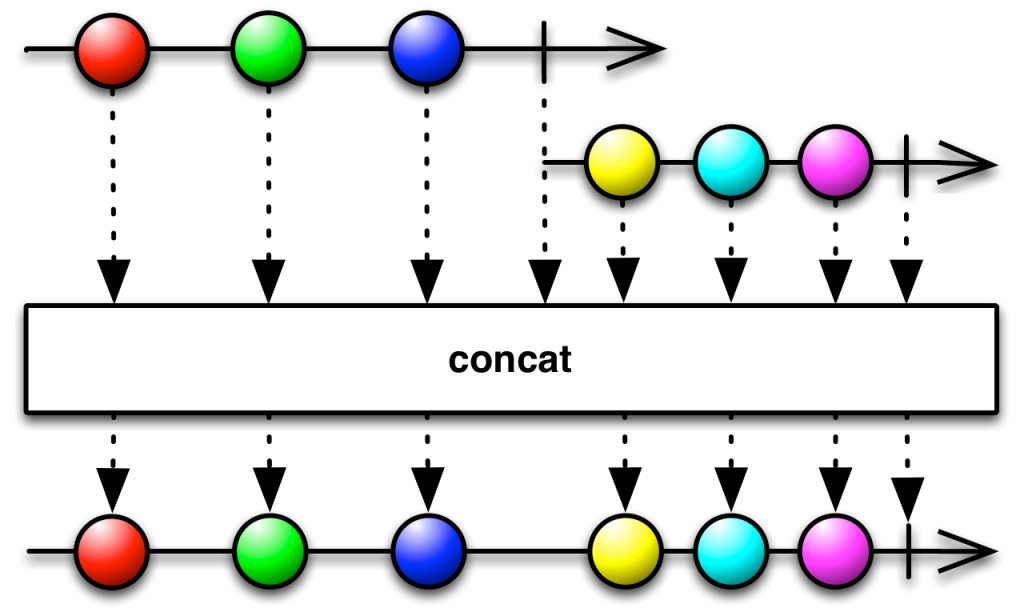
\includegraphics[width=1.0\textwidth,page=1]{gfx/concat}
	\end{figure}
\end{frame}

\begin{frame}{merge()}
	\begin{figure}[h]
		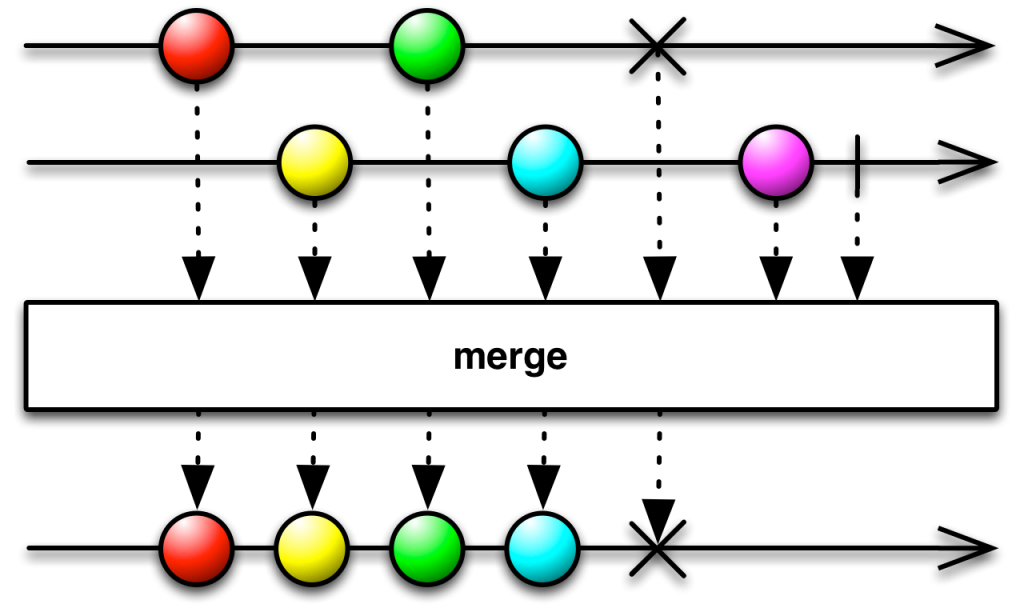
\includegraphics[width=1.0\textwidth,page=1]{gfx/merge}
	\end{figure}
\end{frame}

\begin{frame}{map()}
	\begin{figure}[h]
		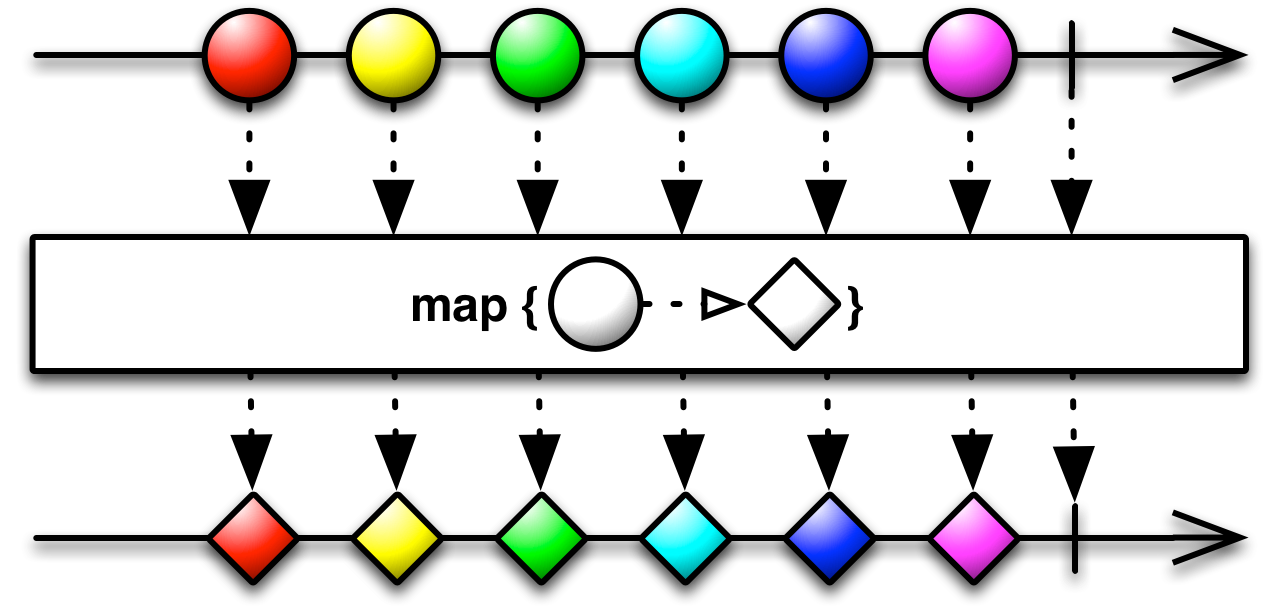
\includegraphics[width=1.0\textwidth,page=1]{gfx/map}
	\end{figure}
\end{frame}

\begin{frame}{filter()}
	\begin{figure}[h]
		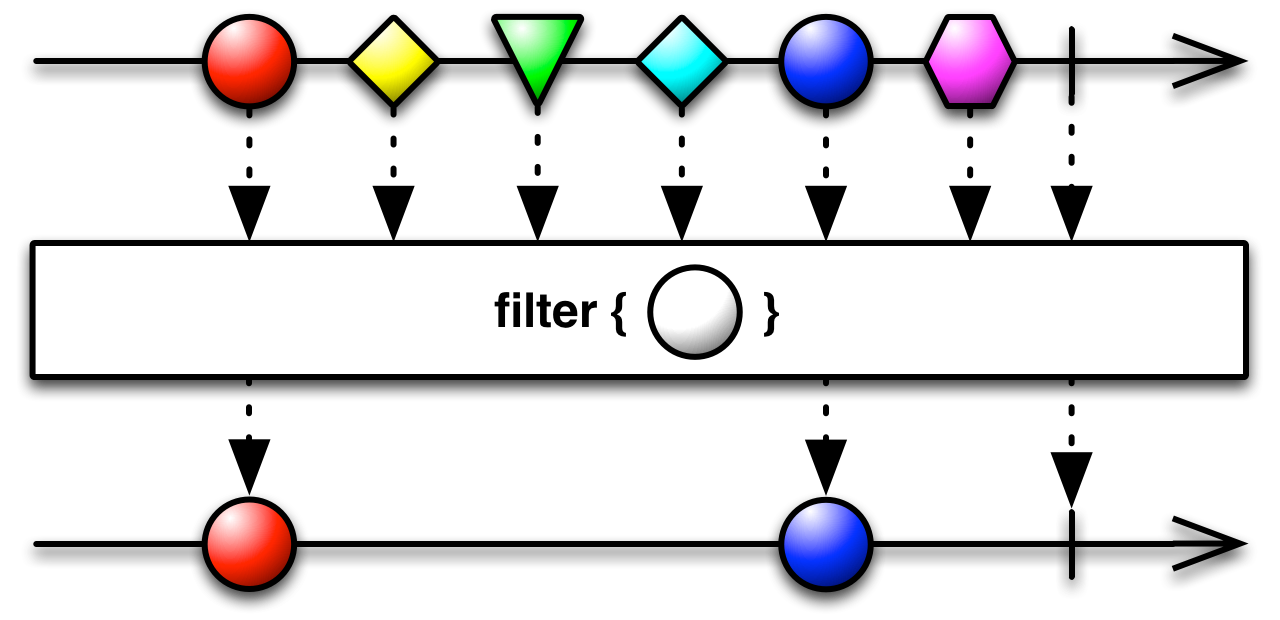
\includegraphics[width=1.0\textwidth,page=1]{gfx/filter}
	\end{figure}
\end{frame}

\begin{frame}{concatMap()}
	\begin{figure}[h]
		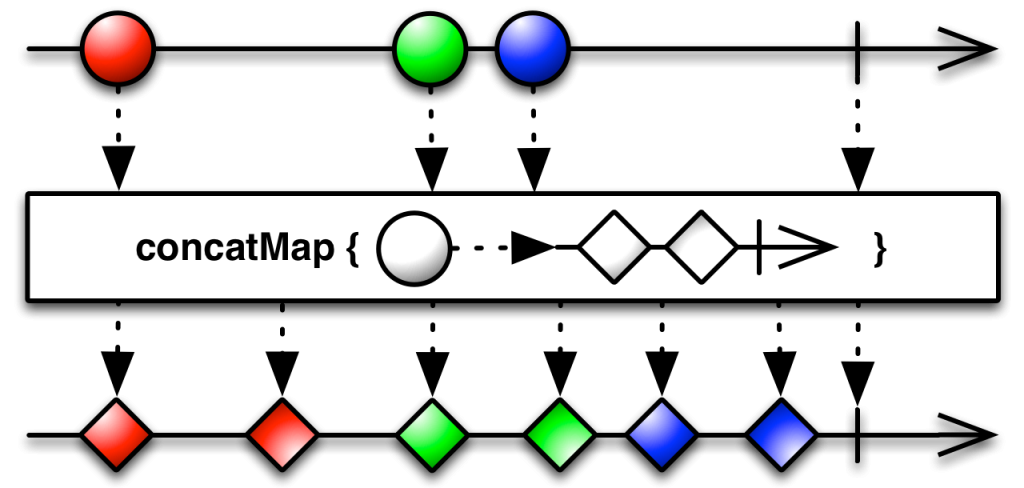
\includegraphics[width=1.0\textwidth,page=1]{gfx/concatMap}
	\end{figure}
\end{frame}

\begin{frame}{flatMap()}
	\begin{figure}[h]
		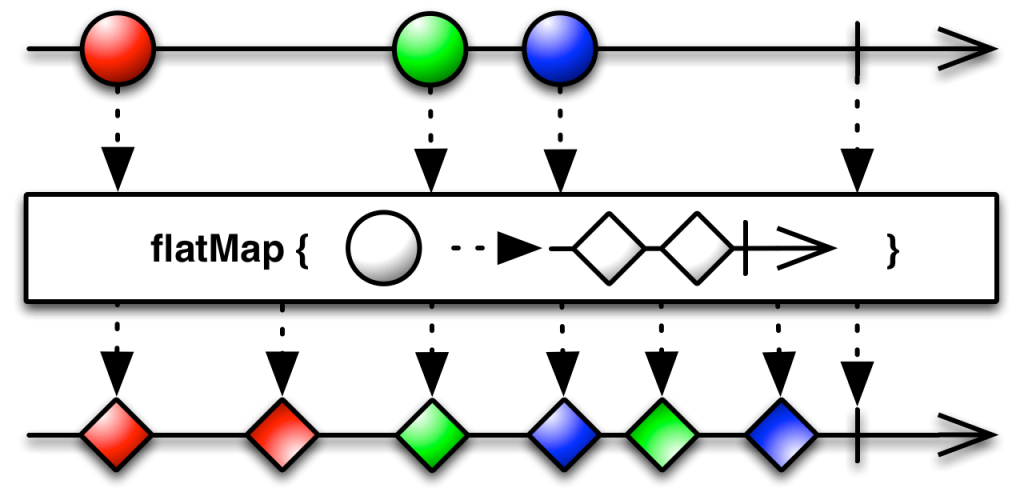
\includegraphics[width=1.0\textwidth,page=1]{gfx/flatMap}
	\end{figure}
\end{frame}

\begin{frame}{reduce()}
	\begin{figure}[h]
		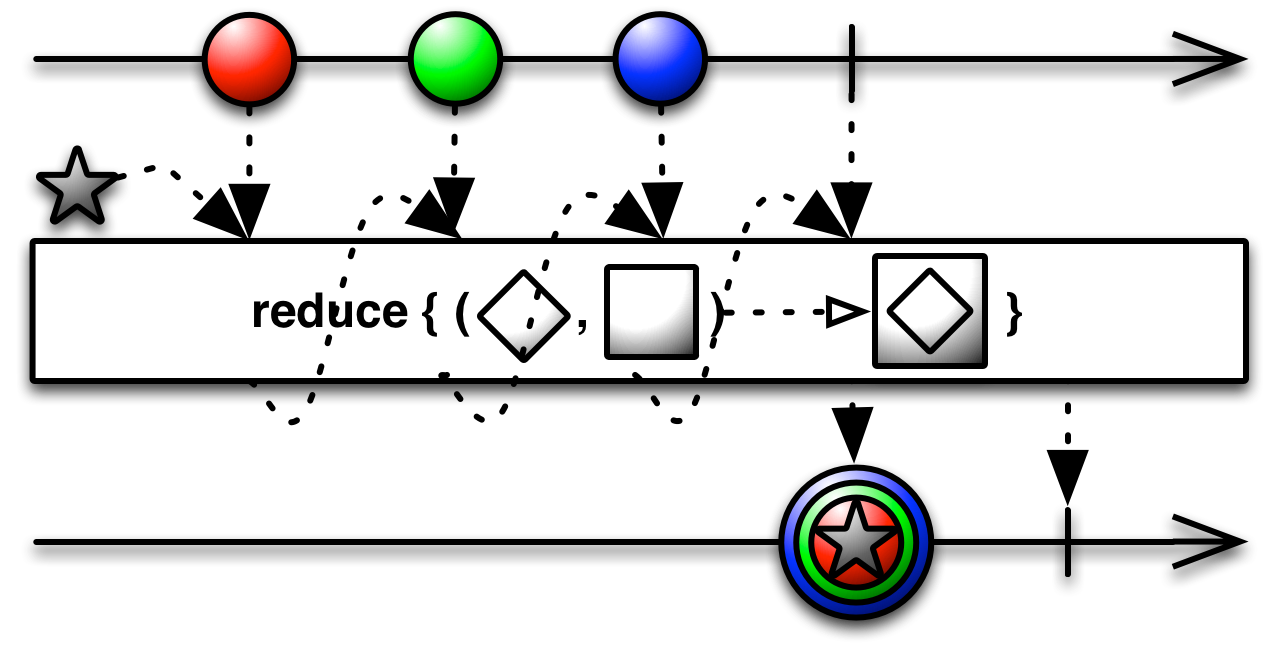
\includegraphics[width=1.0\textwidth,page=1]{gfx/reduce}
	\end{figure}
\end{frame}

\begin{frame}{sum()}
	\begin{figure}[h]
		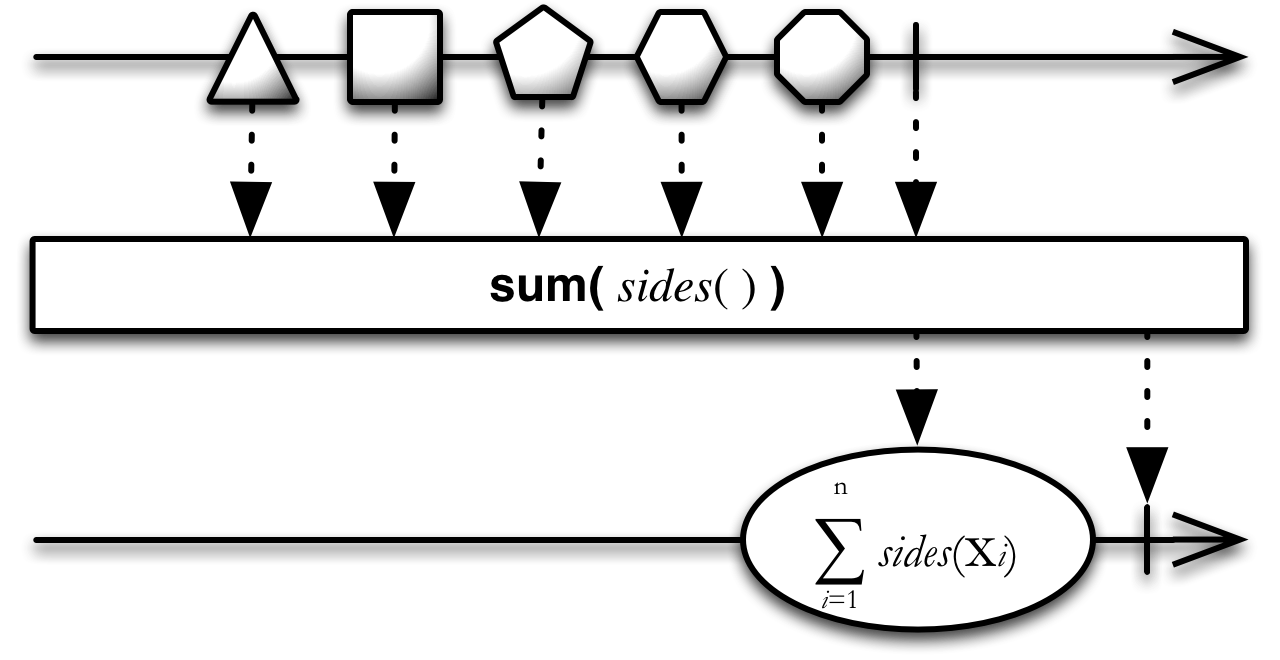
\includegraphics[width=1.0\textwidth,page=1]{gfx/sum}
	\end{figure}
\end{frame}

\begin{frame}{scan()}
	\begin{figure}[h]
		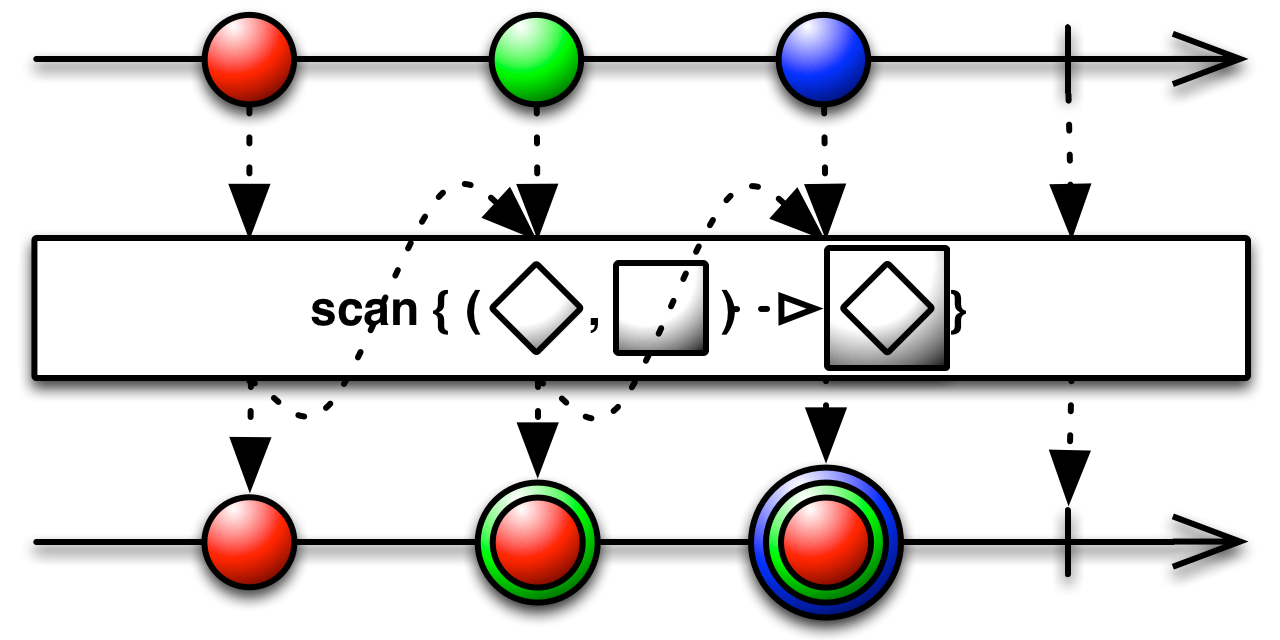
\includegraphics[width=1.0\textwidth,page=1]{gfx/scan}
	\end{figure}
\end{frame}


\section{Task: Donald's Restaurant}\label{sec:donald}

\begin{frame}
	\centering
    \LARGE
    {\nameref{sec:donald}}
\end{frame}

\begin{frame}{A short recap}
    \begin{enumerate}
        \item Orders are submitted as strings in the format: \\
        \enquote{\texttt{<meal\_number>, <servings>}}
        \item Requests for meals are Lists that contain 1 to n Orders
        \item Order strings are split at the comma and used to construct a new Order object
        \item All Orders from one Request are put into an OrderLine object
        \item All Orders in a Request are assigned an increasing index as the order number
        \item Orders are turned into Meals while waiting for a time specified in its recipe
    \end{enumerate}
\end{frame}

\begin{frame}{{\nameref{sec:donald}}}
	\begin{itemize}
		\item Download the zipped project from the workshop repository
        \item Open the project in Netbeans or IntelliJ
        \item Open the class \texttt{Main.java}
	\end{itemize}
    \medskip
    \centering
    \LARGE
    \textbf{\url{https://git.io/vFPQB}}\\
    \normalsize
    \bigskip
    \url{http://reactivex.io/documentation/operators}\\
    RxJava GitHub wiki: \url{https://git.io/vWHZx}\\
    Original Restaurant: \url{https://git.io/vFPby}
\end{frame}

\begin{frame}{{\nameref{sec:donald}}}
    \centering
    \Large
    Create a stream of order strings and print them
\end{frame}

\begin{frame}{{\nameref{sec:donald}}}
    \centering
    \Large
    Parse the order strings into \texttt{Orders} and put them into \texttt{OrderLine}s, then print those
\end{frame}

\begin{frame}{{\nameref{sec:donald}}}
    \centering
    \Large
    Transform every \texttt{Order} in an \texttt{OrderLine} into a \texttt{Meal} and print it
\end{frame}

\begin{frame}{{\nameref{sec:donald}}}
    \centering
    \Large
    Filter out invalid \texttt{Order}s, based on checking their recipe number\\
    Handle exceptions by skipping invalid items
\end{frame}

\begin{frame}{{\nameref{sec:donald}}}
    \centering
    \Large
    Add an incrementing order number to each new \texttt{OrderLine}
\end{frame}

\begin{frame}{{\nameref{sec:donald}}}
	\begin{figure}[h]
		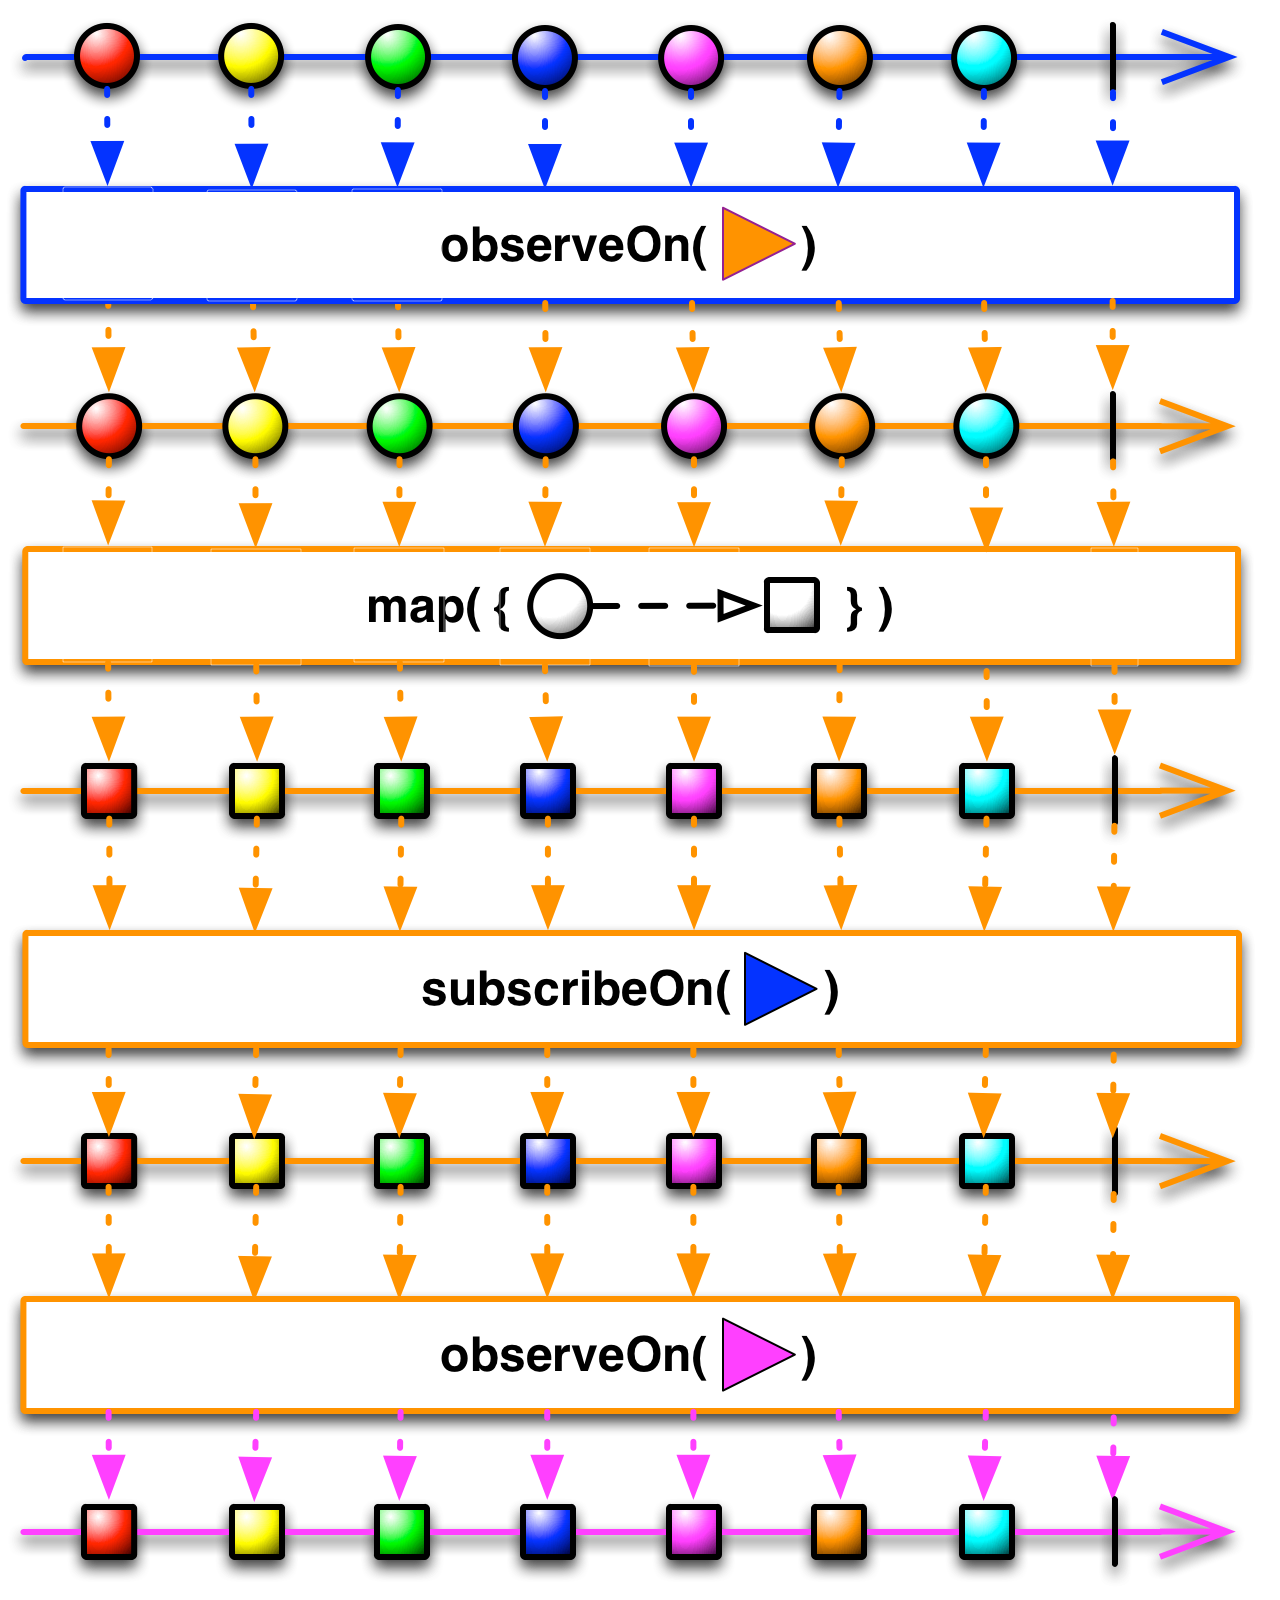
\includegraphics[width=0.6\textwidth,page=1]{gfx/schedulers}
	\end{figure}
\end{frame}

\begin{frame}{{\nameref{sec:donald}}}
	\begin{figure}[h]
		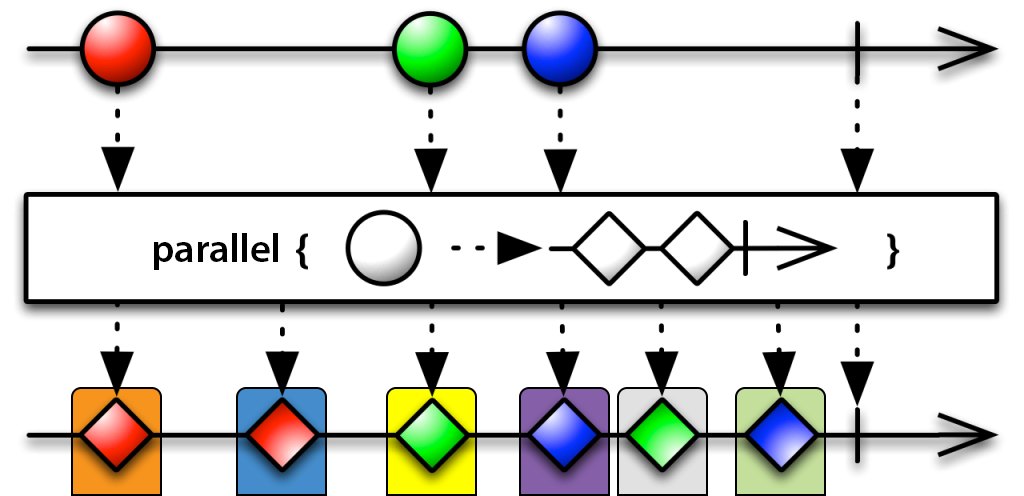
\includegraphics[width=1.0\textwidth,page=1]{gfx/parallel}
	\end{figure}
\end{frame}

\begin{frame}{{\nameref{sec:donald}}}
    \centering
    \Large
    Go multi-threaded by using \texttt{parallel()}
\end{frame}


\section{Backpressure}\label{sec:backpressure}

\begin{frame}{{\nameref{sec:backpressure}}}
    \centering
    \Large
    Hot vs Cold Observables
\end{frame}

\begin{frame}{{\nameref{sec:backpressure}}}
    \begin{itemize}
    	\item \textbf{Cold}: Emit on subscribe(), starting from the beginning
    	\item \textbf{Hot}: Emit constantly, subscribers \enquote{tune} in and out
    \end{itemize}
\end{frame}

\begin{frame}{Backpressure Strategies}
	\begin{itemize}
		\item \textbf{Error}: Signals a MissingBackpressureException. %deadend
        \begin{figure}[h]
			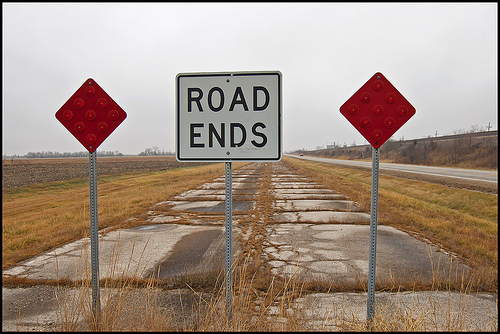
\includegraphics[width=0.8\textwidth,page=1]{gfx/roadend.jpg}
		\end{figure}
    \end{itemize}
\end{frame}

\begin{frame}{Backpressure Strategies}
	\begin{itemize}
    	\item \textbf{Buffer}: Buffers all onNext values. %dam
        \begin{figure}[h]
			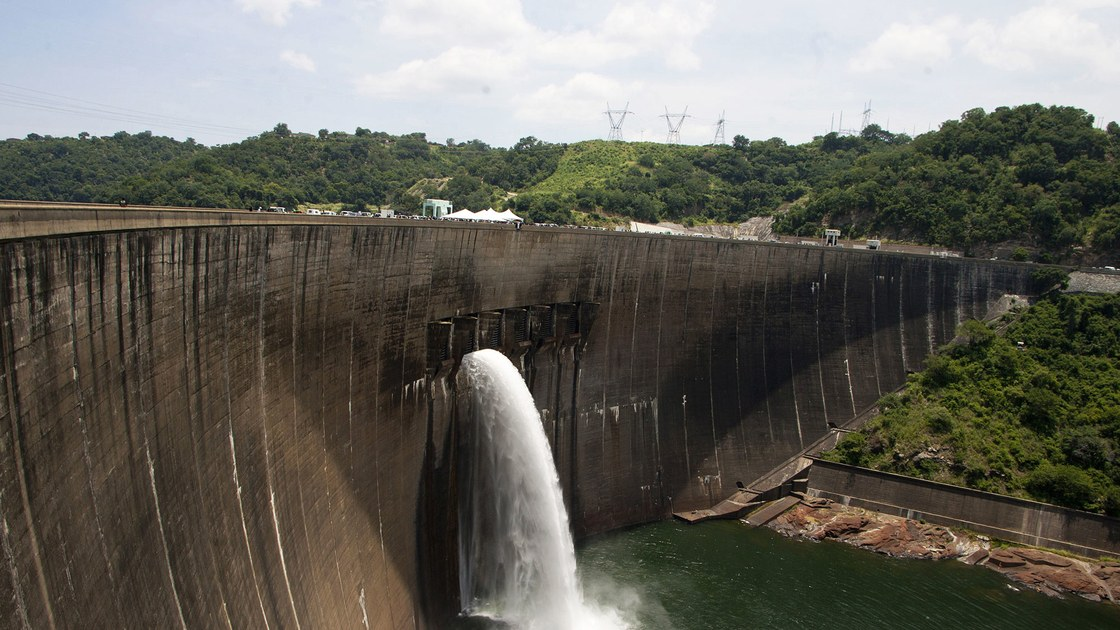
\includegraphics[width=0.9\textwidth,page=1]{gfx/dam.jpg}
		\end{figure}
	\end{itemize}
\end{frame}

\begin{frame}{Backpressure Strategies}
	\begin{itemize}
    	\item \textbf{Drop}: Drops the most recent onNext value. %overflow
        \begin{figure}[h]
			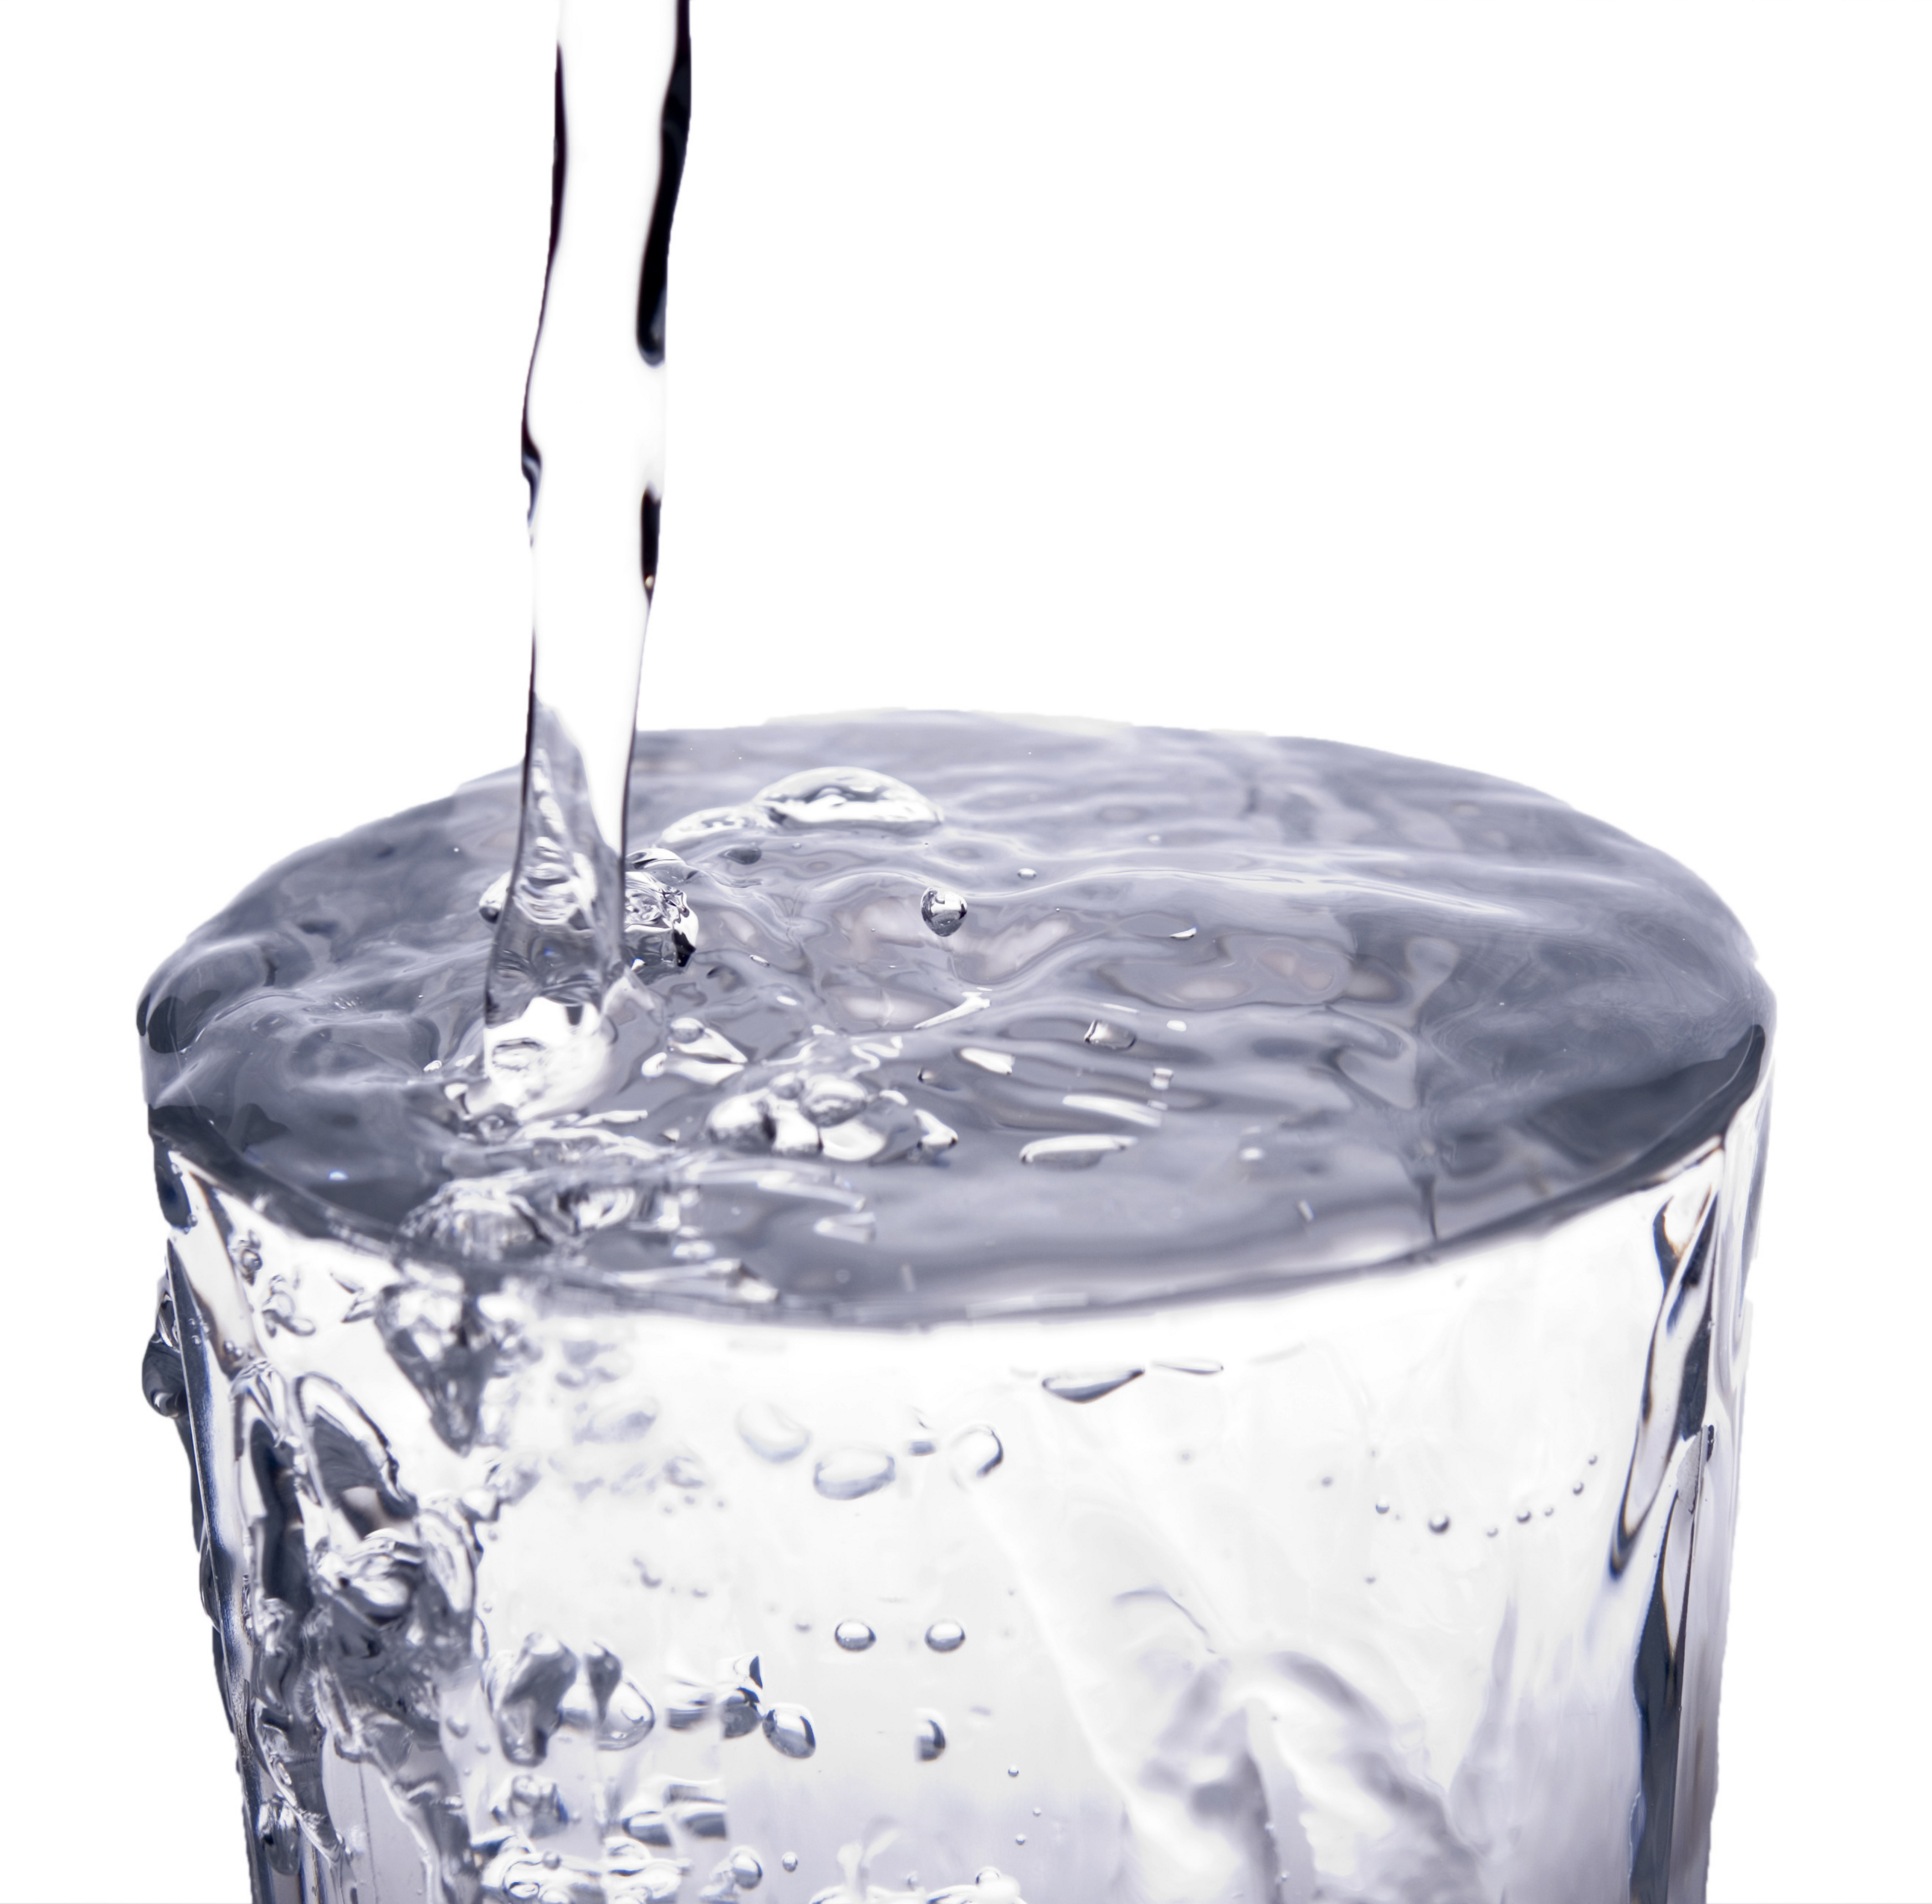
\includegraphics[width=0.6\textwidth,page=1]{gfx/Overflow.jpg}
		\end{figure}
	\end{itemize}
\end{frame}

\begin{frame}{Backpressure Strategies}
	\begin{itemize}
        \item \textbf{Latest}: Keeps only the latest onNext value, overwriting any previous value. %highway exit sign
        \begin{figure}[h]
			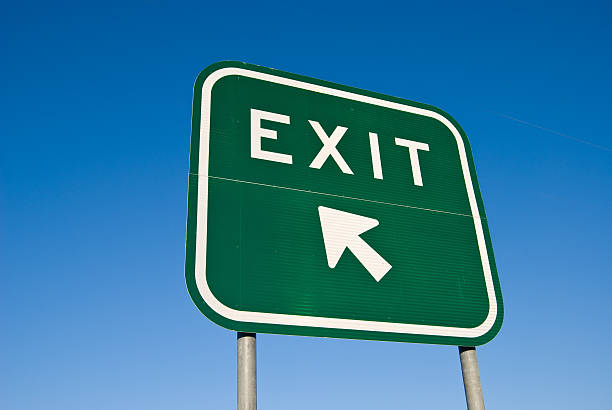
\includegraphics[width=0.8\textwidth,page=1]{gfx/exit.jpg}
		\end{figure}
	\end{itemize}
\end{frame}

\begin{frame}{Backpressure Strategies}
	\begin{itemize}
        \item \textbf{Missing}: OnNext events are written without any buffering or dropping. %no strategy
            \begin{figure}[h]
			
\includegraphics[width=0.7\textwidth,page=1]{gfx/NoStrategy}
		\end{figure}
	\end{itemize}
\end{frame}

%     Backpressure Strategies\\
%     managing hot observables (debounce, sample etc)


\section{TweetStream}\label{sec:tweetstream}

\begin{frame}
	\centering
    \LARGE
    {\nameref{sec:tweetstream}}
\end{frame}

\begin{frame}{{\nameref{sec:tweetstream}}}
	\begin{itemize}
		\item Download the zipped project from the workshop repository
        \item Open the project in Netbeans or IntelliJ
        \item Open the class \texttt{Main.java}
	\end{itemize}
    \medskip
    \centering
    \LARGE
    \textbf{\url{https://git.io/vFPQ8}}\\
    \normalsize
    \bigskip
    \url{http://reactivex.io/documentation/operators}
\end{frame}


% All of the following is optional and typically not needed. 
\appendix
\section<presentation>*{Sources}

\begin{frame}[allowframebreaks]{Sources}
    \begin{thebibliography}{10}

	\setbeamertemplate{bibliography item}[article]

    \bibitem{froussios}
  	Chris Froussios
	\newblock Intro to RxJava
    \newblock \url{https://git.io/vFocj}

    \bibitem{staltz}
    Andre Staltz
	\newblock The introduction to Reactive Programming you've been missing
    \newblock \url{https://git.io/bMkl}

	\setbeamertemplate{bibliography item}[online]

    \bibitem{rx_documentation}
    ReactiveX Documentation
    \newblock Operators \& Getting Started
    \newblock \url{http://reactivex.io/documentation}

    \bibitem{workshop_link}
    RxJava Workshop 2017
    \newblock \url{https://git.io/vFEId}

  \end{thebibliography}
\end{frame}


\end{document}
